\subsection*{Differentialgleichungen}

\begin{example}
Ordnen Sie die folgenden Differentialgleichungen ihren jeweiligen Richtungsfeldern zu:
a. $y^{\prime}=x-y$
b. $y^{\prime}=x-y+1$
c. $2 y y^{\prime}=x$
d. $y y^{\prime}+x=0$
e. $y^{\prime} x+y=0$
f. $y^{\prime}=e^{x-y}$

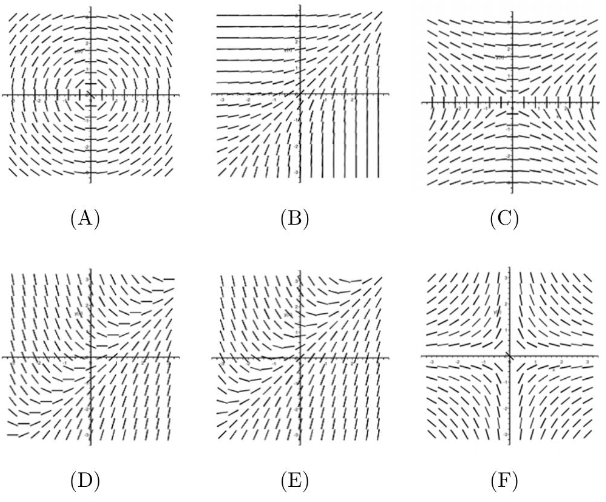
\includegraphics[width=1\linewidth]{images/richtungsfelder.png}

a. Für Werte mit $x=y$ ist die Steigung 0 ; rechts von diesen Wertepaaren ist die Steigung positiv, links davon ist sie negativ. $\Rightarrow$ Bild (D).

b. Die Steigung 0 wird für die Werte mit $y=x+1$ erreicht, ansonsten ist die Situation analog wie bei (a). $\Rightarrow$ Bild (E)

c. Umformen ergibt $y^{\prime}=\frac{x}{2 y}$. Für $x=0$ und $y \neq 0$ ist die Steigung gleich 0 ; für $y=0$ und $x \neq 0$ strebt die Steigung gegen $\infty$. Für die restlichen Werte ist die Steigung ist genau dann positiv, wenn $x$ und $y$ beide das gleiche Vorzeichen haben. $\Rightarrow$ Bild (C)

d. Umformen ergibt $y^{\prime}=-\frac{x}{y}$. Die Situation ist ähnlich wie bei (c), aber die Steigung ist jetzt genau dann positiv, wenn $x$ und $y$ verschiedene Vorzeichen haben. $\Rightarrow$ Bild (A)

e. Umformen ergibt $y^{\prime}=-\frac{y}{x}$. Die Steigung ist 0 für die Werte auf der $x$-Achse mit $x \neq 0$, und sie gehen gegen unendlich für die Werte auf der $y$-Achse mit $y \neq 0 . \Rightarrow$ Bild (F)

f. Für $x=y$ ist die Steigung 1; wenn der $x$-Wert viel grösser als der $y$-Wert ist, dann wird die Steigung sehr gross, im umgekehrten Fall ist sie nahe bei $0 . \Rightarrow$ Bild (B)

\end{example}

\begin{example}
    Wir betrachten das Anfangswertproblem

    $$
    \left\{\begin{aligned}
    y^{\prime} & =\sqrt{x+y} \\
    y(1) & =1
    \end{aligned}\right.
    $$
    
    Bestimmen Sie approximativ $y(1.2)$, d.h. den Wert der Lösungskurve an der Stelle $x=1.2$, durch 4 Schritte (von Hand) mit dem Euler-Verfahren, d.h. mit der Schrittweite $h=0.05$.

\tcblower
Vier Euler-Schritte mit $h=0.05$, d.h. $x_{0}=1, x_{1}=1.05, x_{2}=1.1, x_{3}=1.15, x_{4}=1.2$, und $f(x, y)=\sqrt{x+y}$ :

$$
\begin{aligned}
& y_{0}=1 \\
& y_{1}=y_{0}+h f\left(x_{0}, y_{0}\right) \approx 1.07 \\
& y_{2}=y_{1}+h f\left(x_{1}, y_{1}\right) \approx 1.1435 \\
& y_{3}=y_{2}+h f\left(x_{2}, y_{2}\right) \approx 1.2184 \\
& y_{4}=y_{3}+h f\left(x_{3}, y_{3}\right) \approx 1.2954
\end{aligned}
$$

Insgesamt erhalten wir also die Approximation

$$
y(1.2) \approx 1.2954
$$
\end{example}


\begin{example}
    Finden und klassifizieren Sie die konstanten Lösungen der folgenden Differentialgleichungen: (alles konstante Lösungen)
a. $y^{\prime}=y^{2}-1$
- $y_{1}=-1$ : stabil
- $y_{2}=1$ : instabil

b. $y^{\prime}=y^{2}$
- $y_{1}=0$ : semistabil

c. $y^{\prime}=y^{3}$
- $y_{1}=0$ : instabil

d. $y^{\prime}=-y^{3}$
- $y_{1}=0$ : stabil

\end{example}


\begin{example}
    Lösen Sie mit Separation der Variablen das AWP

    $$
    \left\{\begin{aligned}
    -\dot{N}(t) & =k \cdot N(t) \\
    N(0) & =N_{0}
    \end{aligned}\right.
    $$
    
    des radioaktiven Zerfalls. Dabei ist $N(t)$ die Konzentration zur Zeit $t$ und $N_{0}$ die Konzentration zu Beginn.

\tcblower
Standardform der DGL: $\frac{\mathrm{d} N}{\mathrm{~d} t}=-k \cdot N$. Separation der Variablen:

$$
\int \frac{\mathrm{d} N}{N}=-k \int \mathrm{d} t
$$

also

$$
\ln |N|=-k(t+C)=-k t+\tilde{C}
$$

Auflösen nach $N$ :

$$
N(t)=M \cdot e^{-k t} \quad(M \in \mathbb{R})
$$

Einsetzen der Anfangsbedingung $N(0)=N_{0}$ ergibt $M=N_{0}$, also ist die Lösung des AWPs

$$
N(t)=N_{0} \cdot e^{-k t}
$$
\end{example}





\begin{example}
    Ein Körper besitzt zur Zeit $t=0$ die Temperatur $T_{0}$ und wird in der Folgezeit durch vorbeiströmende Luft der konstanten Temepratur $T_{L}$ gekühlt ( $T_{L}<T_{0}$ ). Der Abkühlungsprozess wird dabei durch die Differentialgleichung

    $$
    \dot{T}=-a\left(T-T_{L}\right) \quad(a>0)
    $$
    
    beschrieben.
    
    a. Bestimmen Sie die zeitliche Entwicklung der Temperatur $T(t)$ des Körpers.
    
    b. Gegen welchen Endwert $\lim _{t \rightarrow \infty} T(t)$ strebt die Temperatur des Körpers?

\tcblower
a. Standardform der DGL: $T^{\prime}=\frac{\mathrm{d} T}{\mathrm{~d} t}=-a\left(T-T_{L}\right)$, also

$$
\int \frac{\mathrm{d} T}{T-T_{L}}=-a \int \mathrm{d} t, \quad \text { integriert: } \quad \ln \left|T-T_{L}\right|=-a t+C, C \in \mathbb{R}
$$

also $\left|T-T_{L}\right|=e^{-a t+C}$ bzw. $T=T_{L} \pm e^{-a t+C}, C \in \mathbb{R}$; die allgemeine Lösung der Gleichung ist damit

$$
T=T_{L}+K \cdot e^{-a t}, \quad K \in \mathbb{R}
$$

(Für $K=0$ ergibt sich die konstante Lösung $T=T_{L}$.) Einsetzen der Anfangsbedingung $T(0)=T_{0}$ ergibt $T_{0}=T_{L}+K$, also $K=T_{0}-T_{L}$, damit ist die gesuchte spezielle Lösung der DGL

$$
T(t)=T_{L}+\left(T_{0}-T_{L}\right) \cdot e^{-a t}
$$

b. Es gilt $\lim _{t \rightarrow \infty} T(t)=T_{L}+\left(T_{0}-T_{L}\right) \cdot \lim _{t \rightarrow \infty} e^{-a t}=T_{L}$ (wegen $a<0$ ), d.h. die Temperatur des Körpers gleicht sich für $t \rightarrow \infty$ der Temperatur der Umgebungsluft an.

\end{example}

\begin{example}
    Bestimmen Sie die allgemeine Lösung der Differentialgleichung
    $
    y^{\prime}=y-7
    $
    auf zwei verschiedene Arten.
\tcblower
a. Lösung mit Separation der Variablen: Standardform der DGL: $y^{\prime}=\frac{\mathrm{d} y}{\mathrm{~d} x}=y-7$, also

$$
\int \frac{1}{y-7} \mathrm{~d} y=\int 1 \mathrm{~d} x, \quad \text { integriert: } \quad \ln |y-7|=x+C, C \in \mathbb{R}
$$

weiter umgeformt: $y-7= \pm e^{x+C}=K \cdot e^{x}$, woei $K= \pm e^{C}$, also ist die allgemeine Lösung der DGL

$$
y=K \cdot e^{x}+7 \quad(K \in \mathbb{R})
$$

b. Lösung mit Variation der Konstanten: Einsetzen in die Lösungsformel $y=$ $e^{-F(x)} \int g(x) e^{F(x)} \mathrm{d} x$ für $g(x)=-7$ und $F(x)=-x$ :

$$
y=e^{x} \int(-7) \cdot e^{-x} \mathrm{~d} x=e^{x}\left(7 e^{-x}+C\right)=C \cdot e^{x}+7 \quad(C \in \mathbb{R})
$$
\end{example}

\begin{example}
    Wir betrachten die Differentialgleichung
$
\dot{N}(t)=k \cdot N(t) \cdot(A-N(t))
$

des Wachstums mit oberer Grenze $A>0$.

a. Bestimmen Sie mit Separation der Variablen die allgemeine Lösung dieser DGL.

b. Bestimmen Sie die spezielle Lösung zum Anfangswert $N(0)=\epsilon>0$ und berechnen Sie den Grenzwert $\lim _{t \rightarrow \infty} N(t)$
\tcblower
a. Standardform der DGL: $\frac{\mathrm{d} N}{\mathrm{~d} t}=k N(A-N)$. Es gibt die konstanten Lösungen $N=0$ und $N=A$; um die übrigen Lösungen zu erhalten, separieren wir die Variablen, also

$$
\int \frac{\mathrm{d} N}{N(A-N)}=k \int \mathrm{d} t
$$

Partialbruchzerlegung von $\frac{1}{N(A-N)}$ :

$$
\frac{1}{N(A-N)}=\frac{1}{A} \cdot \frac{1}{N}+\frac{1}{A} \cdot \frac{1}{A-N}
$$

und damit

$$
\begin{aligned}
\int \frac{\mathrm{d} N}{N(A-N)} & =\frac{1}{A}\left(\int \frac{\mathrm{d} N}{N}+\int \frac{\mathrm{d} N}{A-N}\right)=\frac{1}{A}(\ln |N|-\ln |A-N|)+C \\
& =\frac{1}{A} \ln \left|\frac{N}{A-N}\right|+C
\end{aligned}
$$

also

$$
\frac{1}{A} \ln \left|\frac{N}{A-N}\right|=k t+C \quad(C \in \mathbb{R})
$$

Auflösen nach $N$ :

$$
N(t)=\frac{A C e^{A k t}}{1+C e^{A k t}}=\frac{A}{1+L \cdot e^{-A k t}} \quad(L \in \mathbb{R})
$$

b. Einsetzen der Anfangsbedingung $N(0)=\epsilon$ ergibt $\epsilon=\frac{A}{1+L}$, also $L=\frac{A}{\epsilon}-1$, damit ist die gesuchte spezielle Lösung der DGL

$$
N(t)=\frac{A}{1+\left(\frac{A}{\epsilon}-1\right) e^{-A k t}}
$$

mit $\lim _{t \rightarrow \infty} N(t)=A$ (wegen $A>0$ und $k>0$ gilt $e^{-A k t} \rightarrow 0$ für $t \rightarrow \infty$ ). Dies ist auch von der Anwendung her sinnvoll: Für $t \rightarrow \infty$ nähert sich der Bestand der oberen Grenze $A$ und wächst nicht darüber hinaus.

\end{example}




\begin{example}
    Wir betrachten das Anfangswertproblem

    $$
    \left\{\begin{aligned}
    y^{\prime} & =2 y+x \\
    y(0) & =1
    \end{aligned}\right.
    $$
    
    a. Bestimmen Sie approximativ $y(1)$, d.h. den Wert der Lösungskurve an der Stelle $x=1$, durch 4 Schritte (von Hand) mit dem Euler-Verfahren, d.h. mit der Schrittweite $h=0.25$.
    
    b. Bestimmen Sie analytisch $y(1)$, d.h. bestimmen Sie analytisch die exakte Lösung $y(x)$ und berechnen Sie $y(1)$.

\tcblower
a. Vier Euler-Schritte mit $h=0.25$, d.h. $x_{0}=0, x_{1}=0.25, x_{2}=0.5, x_{3}=0.75, x_{4}=1$, und $f(x, y)=2 y+x$ :

$$
\begin{aligned}
& y_{0}=1 \\
& y_{1}=y_{0}+h f\left(x_{0}, y_{0}\right)=\frac{3}{2}=1.5 \\
& y_{2}=y_{1}+h f\left(x_{1}, y_{1}\right)=\frac{37}{16}=2.3125 \\
& y_{3}=y_{2}+h f\left(x_{2}, y_{2}\right)=\frac{115}{32}=3.59375 \\
& y_{4}=y_{3}+h f\left(x_{3}, y_{3}\right)=\frac{357}{64}=5.578125
\end{aligned}
$$

Insgesamt erhalten wir also die Approximation

$$
y(1) \approx 5.578
$$

b. Um die exakte Lösung zu bestimmen, verwenden wir die Formel $y=e^{-F(x)} \int g(x) e^{F(x)} \mathrm{d} x$ für $g(x)=x$ und $f(x)=-2$, also $F(x)=-2 x$ und (mit partieller Integration)

$$
\begin{aligned}
y & =e^{2 x} \int x \cdot e^{-2 x} \mathrm{~d} x \\
& =e^{2 x}\left(-\frac{1}{4}(2 x+1) e^{-2 x}+C\right) \\
& =-\frac{1}{4}(2 x+1)+C e^{2 x} \quad(C \in \mathbb{R})
\end{aligned}
$$

Einsetzen der Anfangsbedingung $y(0)=1$ ergibt $1=-\frac{1}{4}+C$, also $C=\frac{5}{4}$ und damit die Lösung des AWPs

$$
y=-\frac{1}{4}(2 x+1)+\frac{5}{4} e^{2 x}
$$

Für $x=1$ ergibt sich

$$
y(1)=-\frac{3}{4}+\frac{5}{4} e^{2} \approx 8.486
$$
\end{example}


\begin{example}
    3. Wir betrachten das Anfangswertproblem

    $$
    \left\{\begin{aligned}
    y^{\prime} & =x-y \\
    y(0) & =1
    \end{aligned}\right.
    $$
    
    Gesucht ist $y(2)$, d.h. die Lösung an der Stelle $x=2$.
    
    a. Wir erinnern uns von Serie 11 (Aufgabe 6), dass $y=2 e^{-x}+x-1$ die exakte Lösung des AWPs ist. Berechnen Sie damit $y(2)$.
    
    b. Bestimmen Sie (von Hand) mit dem Euler-Verfahren die approximative Lösung an der Stelle $x=2$ mit den Schrittweiten $h=2, h=1$ und $h=0.5$ (d.h. in 1 Schritt, in 2 Schritten und in 4 Schritten).
    
    c. Führen Sie (mit Software) das Euler-Verfahren mit den Schrittweiten $h=0.1, h=0.01$ und $h=0.001$ aus, um immer bessere Approximationen für $y(2)$ zu erhalten.

\tcblower
a. Die analytisch berechnete Lösung hat an der Stelle $x=2$ also den Wert

$$
y(2)=2 \cdot e^{-2}+1 \approx 1.2707
$$

b. Mit den verschiedenen Schrittweiten ergeben sich folgende Approximationen:
- $h=2: x_{0}=0, x_{1}=2 ; y_{0}=1, y_{1}=-1$, also $y(2) \approx-1$
- $h=1: x_{0}=0, x_{1}=1, x_{2}=2 ; y_{0}=1, y_{1}=0, y_{2}=1$, also $y(2) \approx 1$
- $h=0.5: x_{0}=0, x_{1}=0.5, x_{2}=1, x_{3}=1.5, x_{4}=2 ; y_{0}=1, y_{1}=0.5, y_{2}=0.5$, $y_{3}=0.75, y_{4}=1.125$, also $y(2) \approx 1.125$

c. Mit den verschiedenen Schrittweiten ergeben sich folgende Approximationen:

\begin{tabular}{|c|c|}
\hline Schrittweite $h$ & Approximierter Funktionswert $y(1)$ \\
\hline \hline 0.1 & 1.2432 \\
\hline 0.01 & 1.2680 \\
\hline 0.001 & 1.2704 \\
\hline
\end{tabular}

Man sieht also, dass die Approximation immer besser wird, wenn die Schrittweite verkleinert wird.

\end{example}


\begin{example}
    Wir betrachten das Anfangswertproblem

    $$
    \left\{\begin{aligned}
    y^{\prime} & =\cos (x+y)+\sin (x-y) \\
    y(0) & =0
    \end{aligned}\right.
    $$
    
    Gesucht ist $y(1)$, d.h. die Lösung an der Stelle $x=1$.
    
    b. Führen Sie (von Hand) das Euler-Verfahren mit der Schrittweite $h=0.5$ aus, um in zwei Schritten zur Lösung zu gelangen.
    
    c. Führen Sie (mit Software) das Euler-Verfahren mit den Schrittweiten $h=0.1, h=0.01$ und $h=0.001$ aus, um immer bessere Approximationen für $y(1)$ zu erhalten.

\tcblower
b. Zwei Euler-Schritte mit $h=0.5$, d.h. $x_{0}=0, x_{1}=0.5, x_{2}=1$ und

$$
\begin{aligned}
& f(x, y)=\cos (x+y)+\sin (x-y): \\
y_{0} & =0 \\
y_{1} & =y_{0}+h f\left(x_{0}, y_{0}\right)=0+0.5 \cdot(\cos (0+0)+\sin (0-0))=0.5 \\
y_{2} & =y_{1}+h f\left(x_{1}, y_{1}\right)=0.5+0.5 \cdot(\cos (0.5+0.5)+\sin (0.5-0.5)) \approx 0.770
\end{aligned}
$$

Dies ergibt also die Approximation

$$
y(1) \approx 0.770
$$

c. Mit den verschiedenen Schrittweiten ergeben sich folgende Approximationen:

\begin{tabular}{|c|c|}
\hline Schrittweite $h$ & Approximierter Funktionswert $y(1)$ \\
\hline \hline 0.1 & 0.6718 \\
\hline 0.01 & 0.6558 \\
\hline 0.001 & 0.6542 \\
\hline
\end{tabular}
\end{example}


